Die ReCiPe-Methode ist eine Methode zur Umsetzung einer Wirkungsabschätzung. Sie verwendet 18 Wirkungskategorien auf der „Midpoint-Ebene“ und fasst diese zu 3 Kategorien auf der „Endpoint-Ebene“ zusammen. Die drei Endpoint-Kategorien sind menschliche Gesundheit, Vielfalt der Ökosysteme und Ressourcenverfügbarkeit. Aus diesen drei Endpunkten wird dann ein einzelner Indikator berechnet, welcher in sogenannten „Ecopoints“ (Pt) ausgedrückt wird. Mit diesem Indikator lassen sich verschiedene Produkte bezüglich ihrer Umweltwirkung vergleichen\citebib{goedkoop}{S.2f.}{vgl. }.
Die drei Endpunkte sind als schützenswerte Bereiche deklariert, und haben jeweils einen Indikator, um die Auswirkungen auf diese Bereiche zu messen.\\
Die erste Kategorie, menschliche Gesundheit, verwendet als Indikator die sogenannten disability-adjusted life years (DALY). Auf Deutsch könnte dieser Indikator als verlorene gesunde Lebensjahre übersetzt werden. Beim DALY-Konzept werden die verlorenen Lebensjahre durch Tod oder Behinderung summiert und als Kennzahl dargestellt\citebib{goedkoop}{S.7f.}{vgl. }.\\
Die Vielfalt der Ökosysteme wird durch den Verlust von Spezies in einem Jahr bemessen. Ökosysteme sind sehr komplex und es ist extrem schwierig diese anhand einer Kennzahl abzubilden. Dennoch wird bei der ReCiPe-Methode die Annahme getroffen, dass sich die Qualität eines Ökosystems durch die Vielfalt der Spezies ausreichend bemessen lässt\citebib{goedkoop}{S.8ff.}{vgl. }.\\
Ein großes Problem der Zukunft wird vermutlich sein, dass der Menschheit die Ressourcen ausgehen werden. Dieses Problem wird in der dritten Kategorie, der Ressourcenverfügbarkeit, festgehalten. Hierbei wird die durch die Verwendung von Ressourcen entstehende Grenzkostensteigerung für die zukünftige Extraktion von Ressourcen als Indikator herangezogen. Da eine Erhöhung der Kosten für Öl einen deutlich höheren Einfluss auf die Gesellschaft hat, als die Erhöhung der Kosten für zum Beispiel Quecksilber, werden die Grenzkostensteigerungen für verschiedene Ressourcen unterschiedlich gewichtet. So wird die Schwere der Auswirkungen einer Kostenerhöhung mit einbezogen. Der Indikator wird in Dollar angegeben\citebib{goedkoop}{S.10ff.}{vgl. }.
\FloatBarrier
\begin{figure}[ht!]
    \centering
    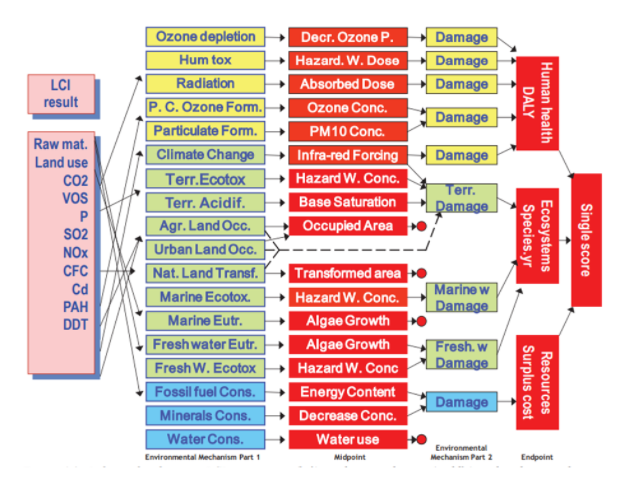
\includegraphics[width=.75\textwidth]{quellen/recipe.png}
    \caption[Zusammenhang der verschiedenen Indikatoren der ReCiPe-Methode]{Zusammenhang der verschiedenen Indikatoren der ReCiPe-Methode (\textit{Geodkoop et al}, S.3)}
\end{figure}
\FloatBarrier